\documentclass[10pt]{article}
\usepackage[utf8]{inputenc}
\usepackage[spanish]{babel}
\usepackage{graphicx}
\usepackage{listings}
\usepackage{hyperref}
\usepackage{amsmath}
\usepackage{float}
\usepackage{cite}
\usepackage{titling}
\usepackage{graphicx}
\setcounter{secnumdepth}{0}
\usepackage{lineno}
\usepackage{tocloft}  % Paquete para manipular el contenido del índice
\usepackage[utf8]{inputenc}  % Para manejar caracteres especiales

\title{Multiplicación de Números de Gran Longitud: Estudio de Métodos de Almacenamiento y Complejidad Temporal}


\author{Gabriel Isaac Valdez Nole\\ \\ Departamento de Matemática \\ y Ciencia de la Computación, \\Universidad de Santiago de Chile, Santiago, Chile}

\date{21 de octubre de 2024}


\begin{document}

\maketitle

\begin{abstract}
En este informe se implementan en lenguaje C tres métodos para almacenar los dígitos de los números de gran longitud a multiplicar de una forma eficiente, con el método clásico dígito a dígito. El primer método almacena cada dígito en 1 byte, el segundo almacena 2 dígitos en un byte, y el tercero convierte el número a base 256. Cabe recalcar que el arreglo que contiene los resultados tiene la misma composición, respectivamente. Se analiza la complejidad temporal y espacial de cada método y se presentan experimentos que comparan su rendimiento.
\end{abstract}

\section{Introducción}
La multiplicación de números de gran longitud es un problema fundamental en el campo de la computación y tiene aplicaciones en criptografía, análisis numérico y otros campos, según la fuente \cite{X1}. Este informe analiza tres métodos para multiplicar números grandes en un tamaño máximo de 1024 bytes, el cual se usará para almacenar la memoria de los punteros que se asignan para resolver el problema de la multiplicación de números de gran longitud, y analiza su complejidad temporal.\\\
La estructura de este informe constará de la siguiente manera: comenzamos con un acercamiento al tema con el abstract, seguimos con una introducción para más profundidad del tema, continuamos con un desarrollo en el cual se presentan los fundamentos de la multiplicación dígito a dígito, explicación del algoritmo, implementación de las funciones más importantes en lenguaje C, correctitud del programa, análisis de la complejidad temporal y espacial de los distintos métodos, experimentos y resultados, para finalmente terminar con una conclusión.

\section{Desarrollo}
Se comenzará explicando los fundamentos de la multiplicación, el método clásico de la multiplicación y se darán detalles sobre cómo se manejó la implementación en lenguaje C.

\subsection{Multiplicación de números enteros}

Sean $a$ y $b$ dos números enteros donde $a \neq 0$. Entonces:

\[
ab = b + b + \cdots + b \quad \text{(a sumandos)}
\]

Si $a = 1$, entonces $ab = 1 \cdot b = b$; también $0 \cdot b = 0$ para todo $b$.

\medskip

Dado que la multiplicación combina dos números para formar un único número, es una operación binaria \cite{X3}.

\subsection{Explicación del algoritmo de la multiplicación dígito a dígito}

Se comenzará con un ejemplo. Primero se multiplicarán los números 123 y 56. La multiplicación se hace dígito a dígito, empezando desde la derecha hacia la izquierda del multiplicando.

\subsection*{Paso 1: Multiplicar 123 por 6 (el primer dígito de derecha a izquierda)}

\[
\begin{array}{r}
     123 \\
  \times 6 \\
  \hline
     738
\end{array}
\]

Multiplicamos cada dígito de 123 por 6:

\begin{itemize}
    \item $6 \times 3 = 18$, se guarda como primer dígito del primer resultado el 8 y se almacena el 1 como acarreo.
    \item $6 \times 2 = 12$, se suma el acarreo al resultado actual, se obtiene 13. Se guarda el 3 como segundo dígito del primer resultado y se guarda el 1 como acarreo.
    \item $6 \times 1 = 6$, se suma el acarreo al resultado actual, se obtiene 7. Se guarda como tercer dígito del primer resultado.
\end{itemize}

El resultado de esta multiplicación es 738.

\subsection*{Paso 2: Multiplicar 123 por 5 (el segundo dígito de derecha a izquierda)}

Ahora se multiplica 123 por 5. Como 5 está en la segunda posición de derecha a izquierda, el resultado debe desplazarse una posición hacia la izquierda (agregamos un 0 al final):

\begin{itemize}
    \item $5 \times 3 = 15$, se guarda como primer dígito del segundo resultado el 5 y se almacena el 1 como acarreo.
    \item $5 \times 2 = 10$, se suma el acarreo al resultado actual, se obtiene 11. Se guarda el 1 como segundo dígito del segundo resultado y se guarda el 1 como acarreo.
    \item $5 \times 1 = 5$, se suma el acarreo al resultado actual, se obtiene 6. Se guarda como tercer dígito del segundo resultado.

    (En caso de que el último resultado dé un número de 2 dígitos, se almacenan ambos dígitos en el mismo orden de la multiplicación.)
\end{itemize}

El resultado es 6150.

\subsection*{Paso 4: Sumar los resultados parciales obtenidos.}

Finalmente, se suman los resultados parciales:

\[
\begin{array}{r}
     738 \\
    + 6150 \\
  \hline
      6888
\end{array}
\]

Por lo tanto, el producto de 123 por 56 es:

\[
123 \times 56 = 6888
\]

\subsection{Descripción del Código}

El código utilizado en este experimento implementa tres métodos de almacenamiento de dígitos para multiplicar números de gran longitud de manera eficiente:

\begin{enumerate}
    \item \textbf{Un dígito por byte}: Cada dígito de los números a multiplicar se almacenará en 1 byte. Se usará el tipo de dato unsigned char, ya que este tipo de dato usa 1 byte, según la fuente \cite{X4}. La implementación se basa en recorrer ambos arreglos con un doble for. Primero se extraen los dígitos del arreglo en una variable int para poder hacer la operación de multiplicación dígito a dígito. Aunque no se usará ningún arreglo extra para mantener los resultados parciales, ya que se almacenarán en el resultado de forma inmediata, el caso donde el resultado tenga 2 dígitos se manejará de la siguiente forma: se guarda el número de 2 dígitos con operaciones de módulo 10, se extraen los dígitos y se almacenan en el arreglo final. La siguiente iteración será multiplicar los dígitos que siguen, al resultado de los dígitos se le suma el acarreo que se tenía en la variable int, extrayendo el dígito con una división entre 10. Esto se repite con todos los números del arreglo para finalmente mostrar el resultado, el cual tendrá bytes iguales a la suma de la cantidad de dígitos de ambos números más 1.
    
    \item \textbf{Dos dígitos por byte}: Cada 2 dígitos de los números se almacenarán en 1 byte. Se usará el tipo de dato unsigned char, como en el caso anterior. La diferencia es que, sabiendo que 1 byte es igual a 8 bits, se tomarán los 4 bits menos significativos y los 4 bits más significativos para guardar 2 dígitos del número en 1 byte. Esto es posible realizando operaciones de desplazamiento de bits. Primero realizamos una operación de \& con el dígito actual y "00001111" para acceder a los bits menos significativos, y para acceder a los bits más significativos simplemente desplazamos $\ll$ 4 espacios. Usando esta metodología y manejando los arreglos con un doble for anidado, se multiplican los dígitos accediendo a los bits. Pero en este caso se necesita una función que calcule la posición donde se almacenará el resultado porque, al acceder a los bits, es necesario calcular la posición correcta para sumar los resultados parciales. Esto se realiza sumando la posición actual del primer número y la posición actual del segundo número. Una vez ubicada la posición, se tiene una función que coloca los dígitos empaquetados en el resultado, para no tener que recurrir a un arreglo extra para almacenar los resultados parciales. Se repite con todos los dígitos del arreglo. Finalmente, si la última multiplicación tiene un acarreo, con un ciclo while se busca la posición y después se empaqueta a nivel de bits. En este caso, el resultado tendrá bytes iguales a la suma de la cantidad de dígitos de ambos números + 1 dividido entre 2.
    Adicionalmente, si el largo de los números es impar, se almacenará el dígito restante en los 4 bits más significativos y en los 4 bits menos significativos se colocará un cero. Este cero tiene una condición: si el número es de largo impar, no se toma en cuenta el dígito menos significativo en la última iteración.
    
    \item \textbf{Base 256}: Cada uno de los números se guardará en 1 byte. Se usará el tipo de dato unsigned char. En este caso, se aprovechará al máximo el espacio, logrando almacenar números de hasta $2^8 - 1$, ya que se usará la base 256. En este caso, sí se usará un arreglo temporal para los resultados parciales, ya que al trabajar con una base mayor, la cantidad de dígitos se reduce. El tamaño del arreglo que contendrá el número en base decimal se logra sacar gracias a un contador que va iterando cada vez que se guarda un número en base 256 en cada espacio del arreglo temporal. De esta forma, se asigna la memoria al arreglo que tendrá el número en base 256 con este contador. Para asignar la memoria desde una función, se usa un doble puntero.
    En el caso de la función de multiplicar, se maneja con un doble for para iterar los arreglos en base 256. En este caso, igualmente se usará una variable temporal, porque se aplicará lo mismo que se usó para almacenar el número en base 256. Primero se asigna un int para el acarreo con un valor de cero cada vez que se mueve el primer número. Seguimos asignando un índice auxiliar para saber la posición en la cual se asignará el resultado en base 256. Después de operar dígito a dígito sumando su acarreo correspondiente en su posición correspondiente (que es la suma de las posiciones de los números que se están operando), seguimos dividiendo entre 256 para obtener el resto, el cual se almacena en la siguiente posición del arreglo. Repetimos este paso hasta terminar el arreglo. Finalmente, se tiene un ciclo while para calcular el largo real del resultado, eliminando los ceros de la izquierda y almacenando el resultado final en el arreglo correspondiente.
\end{enumerate}

A continuación, se presentarán las funciones más importantes del código utilizado para el experimento. En los siguientes fragmentos de código se basará el cálculo de la complejidad temporal y espacial en la sección 2.5:

\lstset{
    basicstyle=\ttfamily\footnotesize,
    breaklines=true,
    breakatwhitespace=true,
    numbers=left,
    numberstyle=\tiny,
    stepnumber=1,
    numbersep=5pt,
    keywordstyle=\color{blue},
    commentstyle=\color{gray},
    showstringspaces=false
}

\begin{lstlisting}
void multiply1digbyte(unsigned char *num1, unsigned char *num2, unsigned char *resultado1digbyte,unsigned int len1,unsigned int len2) {

    unsigned int digit1,digit2,product;
    int i,j;

    for (i = 0; i < len1 + len2+1; i = i + 1) {
        resultado1digbyte[i] = 0;
    }

    for ( i = len1 - 1; i >= 0; i = i - 1) {
        for ( j = len2 - 1; j >= 0; j = j - 1) {

            digit1 = num1[i] - '0'; 
            digit2 = num2[j] - '0'; 

            product = digit1 * digit2 + resultado1digbyte[i + j + 1]; 
            resultado1digbyte[i + j + 1] = product % 10; 
            resultado1digbyte[i + j] = resultado1digbyte[i + j] + product / 10;

        }
    }
}

void multiply2digbyte(unsigned char *num1, unsigned int len1_digitos, unsigned char *num2, unsigned int len2_digitos, unsigned char *resultado) {
    unsigned int lenres_digitos, lenres_bytes, carry, sum, posicion;
    unsigned char digit1, digit2, res_digit;
    int i, j;

    lenres_digitos = len1_digitos + len2_digitos;
    lenres_bytes = (lenres_digitos + 1) / 2;

    for (i = 0; i < lenres_bytes; i = i + 1) {
        resultado[i] = 0;
    }

    for (i = 0; i < len1_digitos; i = i + 1) {

        digit1 = buscar_posicion_digito(num1, len1_digitos, i);
        carry = 0;

        for (j = 0; j < len2_digitos; j = j + 1) {

            digit2 = buscar_posicion_digito(num2, len2_digitos, j);
            posicion = i + j;
            sum = digit1 * digit2 + buscar_posicion_digito(resultado, lenres_digitos, posicion) + carry;
            res_digit = sum % 10;
            carry = sum / 10;
            colocar_digito(resultado, lenres_digitos, posicion, res_digit);

        }
        posicion = i + len2_digitos;

        while (carry > 0) {

            sum = buscar_posicion_digito(resultado, lenres_digitos, posicion) + carry;
            res_digit = sum % 10;
            carry = sum / 10;
            colocar_digito(resultado, lenres_digitos, posicion, res_digit);
            posicion = posicion + 1;

        }
    }
}

void multiply_base256(unsigned char *num1, unsigned int len1, unsigned char *num2, unsigned int len2, unsigned char **resultado, unsigned int *len_res, double *required_memory256) {
    unsigned int lenres, carry, indiceaux, product;
    unsigned char *temp;
    int i, j, indice;

    lenres = len1 + len2;
    temp = (unsigned char *)calloc(lenres, sizeof(unsigned char));

    for (i = 0; i < len1; i = i + 1) {
        carry = 0;

        for (j = 0; j < len2; j = j + 1) {
            indiceaux = i + j;
            product = (unsigned int)num1[len1 - 1 - i] * (unsigned int)num2[len2 - 1 - j] + temp[indiceaux] + carry;
            temp[indiceaux] = (unsigned char)(product % 256);
            carry = product / 256;
        }

        temp[i + len2] = temp[i + len2] + carry;
    }

    indice = lenres;

    while (indice > 0 && temp[indice - 1] == 0) {
        indice = indice - 1;
    }

    *len_res = indice;
    *resultado = (unsigned char *)calloc(*len_res, sizeof(unsigned char));
    *required_memory256 = *required_memory256 + (*len_res) * sizeof(unsigned char);

    for (i = 0; i < *len_res; i = i + 1) {
        (*resultado)[i] = temp[*len_res - i - 1];
    }

    free(temp);
}
\end{lstlisting}

\subsection{Correctitud de la implementación en lenguaje C (en el peor caso)}

En este ámbito, para comprobar que los resultados sean correctos, primero se probó con números de una longitud de 10-5 dígitos, con el peor caso donde las longitudes son iguales y el valor de los dígitos es el valor más alto que puede tomar la base decimal, el cual es 9. \\
Con estos casos se llegó a la conclusión de que el resultado de multiplicar 2 números con puros dígitos iguales a 9, con la misma longitud, está dado por una expresión. Se presentará un ejemplo: se tiene como N la longitud de los números a multiplicar. \\

Por consiguiente, el resultado tendrá la siguiente forma:
\([9]^{N-1}\)\([8]^{1}\)\([0]^{N-1}\)\([1]^{1}\)\\

Por lo tanto, si el resultado en peor caso cumple esta expresión, donde cada número aparece las veces a las cuales está elevado, se comprueba que el resultado de la función implementada es correcto. Se analizó un resultado correcto solo en el peor caso porque este fue el caso que se usó para realizar los experimentos.

\subsection{Análisis de Complejidad Temporal y Espacial}

Se analizará la complejidad temporal y espacial de cada método, usando la multiplicación clásica dígito a dígito.

\subsubsection{Método 1: Un Dígito por Byte}

En este método, se almacenará cada dígito en 1 byte. La complejidad temporal es $O(n \times m)$, donde $n$ y $m$ son las longitudes de los números. Se fundamenta en el código, al tener un doble for anidado, el cual se obtiene resolviendo una doble sumatoria, donde los límites son los extremos del for exterior y del for interior. Aunque el peor caso es que los números tengan la misma longitud, sería de $O(n^2)$. \\
En el caso de la complejidad espacial, referenciada a la implementación que se planteó, donde N es el largo del número en el peor caso, será: \\\\
Tres \texttt{unsigned int} (\texttt{digit1}, \texttt{digit2}, \texttt{product}) ocupan:
\[
3 \times 4 = 3 \times 4 \, \text{bytes} = 12 \, \text{bytes}
\]
\texttt{num1} = \(N \, \text{bytes}\) \\
\texttt{num2} = \(N \, \text{bytes}\) \\
\texttt{resultado1digbyte} = (N + N + 1) \times 1 = 2N + 1 \, \text{bytes}

\[
\text{Memoria total} = 12 + N + N + 2N + 1 = 4N + 13 \, \text{bytes}
\]

\subsubsection{Método 2: Dos Dígitos por Byte}

Este método optimiza el almacenamiento al empaquetar dos dígitos en un byte. Aunque reduce el espacio utilizado, la complejidad temporal sigue siendo $O(n \times m)$, ya que el número de multiplicaciones no cambia, ya que tiene la misma cantidad de dígitos que el caso de 1 dígito por byte. Finalmente, recalcamos lo mismo: el peor caso será de $O(n^2)$, si la longitud de los números es la misma.

En el caso de la complejidad espacial será, referenciada a la implementación que se planteó. Donde N es el largo del número en el peor caso, será:  \\\\
Cinco \texttt{unsigned int} (\texttt{lenres\_digitos}, \texttt{lenres\_bytes}, \texttt{carry}, \texttt{sum}, \texttt{posicion}) ocupan:
\[
5 \times 4 = 5 \times 4 \, \text{bytes} = 20 \, \text{bytes}
\]
Tres \texttt{unsigned char} (\texttt{digit1}, \texttt{digit2}, \texttt{res\_digit}) ocupan:
\[
3 \times 1 = 3 \times 1 \, \text{bytes} = 3 \, \text{bytes}
\]
\texttt{num1} = \(\frac{N + 1}{2}  \, \text{bytes}\) \\
\texttt{num2} = \(\frac{N + 1}{2} \, \text{bytes}\) \\
\texttt{resultado1digbyte} = \(\frac{(N + 1)}{2} + \frac{(N + 1)}{2} + 1 = N + 2 \, \text{bytes}\)

\[
\text{Memoria total} = \frac{(N + 1)}{2} + \frac{(N + 1)}{2} + \frac{(N + 1)}{2} + \frac{(N + 1)}{2} + 1 + 20 + 3 = 2N + 26 \, \text{bytes}
\]

\subsubsection{Método 3: Base 256}

Al convertir los números a base 256, se reduce el número de dígitos necesarios para representar el número, lo cual disminuye el número de operaciones. Sin embargo, las operaciones en base 256 son más costosas computacionalmente. La complejidad temporal es aproximadamente $O(n \times m)$. Siguiendo el mismo caso, se puede ver que, aunque la cantidad de dígitos haya disminuido, eso no influirá en lo que a complejidad temporal teórica se refiere; tendrá una complejidad de $O(n^2)$, ya que igualmente se usan 2 for anidados para manejar los arreglos que contienen el número en base 256.\\

En el caso de la complejidad espacial será:\\
Cuatro \texttt{unsigned int} (\texttt{lenres}, \texttt{carry}, \texttt{indiceaux}, \texttt{product}) ocupan:
\[
4 \times 4 = 4 \times 4 \, \text{bytes} = 16 \, \text{bytes}
\] \\
Un \texttt{int} (\texttt{indice}) ocupa:
\[
1 \times 4 = 1 \times 4 \, \text{bytes} = 4 \, \text{bytes} \\
\] \\
Esta variable se usará para recorrer el arreglo temporal, para contar la longitud del resultado en base 256, eliminando posiciones con un valor de cero hasta el primer número distinto de cero que se encuentre. Se denotará como $\alpha$, ya que varía según el largo del número.\\\\
\texttt{num1} = \(N \, \text{bytes}\) \\
\texttt{num2} = \(N \, \text{bytes}\) \\
\texttt{num1\_base256} = ((2/3) x N + 1)) \text{bytes} \\
\texttt{num2\_base256} = ((2/3) x N + 1)) \text{bytes} \\\\
\texttt{temp} = (N + N)\text{bytes}, aunque esta variable se usa solo en la función multiply\_base256, pero se hace un free finalizando la función. Por lo que para este experimento no se contabilizó esta variable. \\\\
\texttt{resultado\_base256} = ((2/3) x N + 1) + (2/3) x N + 1) - $\alpha$ ) \text{bytes} \\\\
Como se mencionó anteriormente, se evitará sumar el espacio de la variable temporal (N + N).\\
En el caso de la memoria final, no se sumará el arreglo temporal, ni tampoco el arreglo que contiene el número en base decimal, ya que en la función multiply\_base256 no es necesario.

\begin{multline*}
\text{Memoria total} = \left(\frac{2}{3} \times N + 1\right) + \left(\frac{2}{3} \times N + 1\right) + \left(\frac{2}{3} \times N + 1\right) \\
+ \left(\frac{2}{3} \times N + 1\right) - \alpha + 16 + 4 \\
= \frac{8}{3}N - \alpha + 22
\end{multline*}\\
En el ámbito de la complejidad temporal teórica, es la misma, pero como se mencionó, el método de base 256 debería ser más rápido porque tiene que realizar menos multiplicaciones, ya que la cantidad de dígitos se reduce al poder representar un dígito en el rango de [0-255]. En términos de espacio, se podría utilizar 4 bits para cada número con operaciones de desplazamiento de bits, pero se necesitarían 12 bits, el cual es equivalente a 1,5 bytes. A diferencia del número en base 256, ya que este mismo número en base decimal se puede almacenar en 1 byte, porque en 1 byte se tienen 8 bits, por lo que el número máximo que se puede almacenar sería $2^8 - 1$. Teniendo esto en cuenta, la cantidad de memoria se reducirá, lo cual se respalda por la fórmula presentada anteriormente, con N el largo en base decimal (2/3 x N + 1) - $\alpha$, siendo $\alpha$ el contador de posiciones donde el dígito es igual a 0.

\subsection{Experimentos y Resultados}

Se realizaron experimentos para medir el tiempo de ejecución y la memoria en bytes de cada método. Para analizar estos datos se hicieron los gráficos \ref{fig:ti1} que mide tiempo de ejecución vs cantidad de dígitos en base decimal, y \ref{fig:me1} que mide memoria usada vs cantidad de dígitos en base decimal. Para realizar este experimento se usaron diferentes tamaños de entrada, tomando en cuenta siempre el peor caso, donde el número contiene puros dígitos con valor 9 y la longitud de los números es la misma.

\begin{figure}[H]
    \centering
    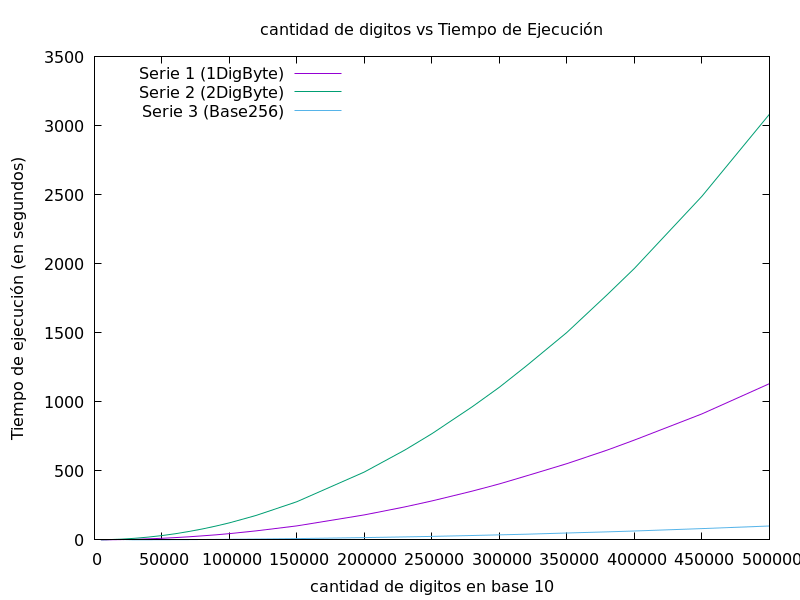
\includegraphics[width=0.8\textwidth]{tiempoDeEjecuccion.png}
    \caption{Tiempo de ejecución vs Cantidad de dígitos}
    \label{fig:ti1}
\end{figure}


\begin{figure}[H]
    \centering
    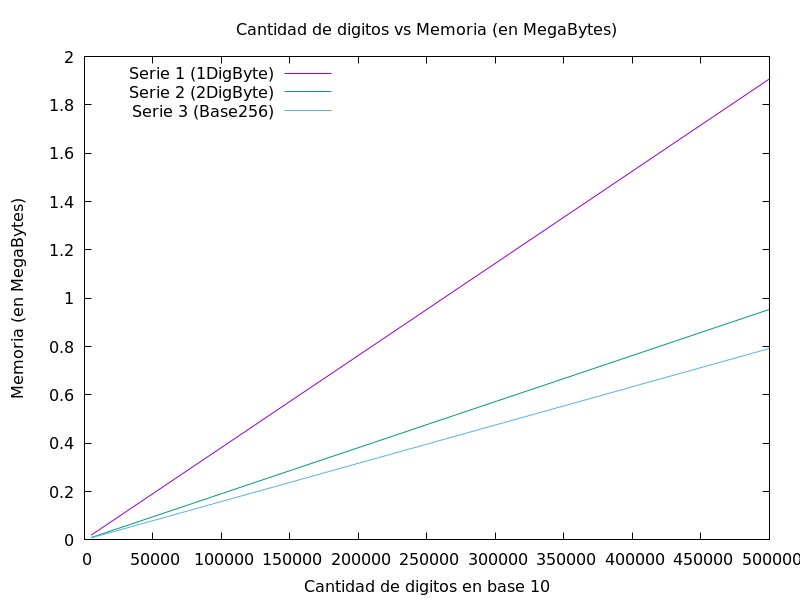
\includegraphics[width=0.8\textwidth]{MemoriaMegabytes.png}
    \caption{Memoria usada vs Cantidad de dígitos}
    \label{fig:me1}
\end{figure}

Gracias a los resultados presentados por los gráficos, se puede ver visualmente lo que teóricamente se presentó anteriormente. Si bien todos los algoritmos pertenecen a la clase de complejidad cuadrática, el crecimiento en cuanto a eficiencia temporal es mucho menor usando el método de la base 256, ya que permite reducir la cantidad de dígitos, lo cual se respalda por el gráfico que muestra como el uso de memoria en el método de la base 256 es mucho menor. Esto permite realizar un cálculo más rápido porque se realizarán menos multiplicaciones. Por otro lado, el método donde se guardan 2 dígitos en 1 byte muestra que este método es más eficiente en temas de memoria que el primer método donde se almacena 1 dígito por byte, pero el tiempo de ejecución se eleva, ya que hay que tener en cuenta que se necesitan hacer operaciones de desplazamiento de bits, buscar posiciones para almacenar a nivel de bits, entre otras, lo que incrementa el tiempo de ejecución. 

Finalmente, se puede observar que el método más eficiente en cuanto a tiempo y uso de memoria sería el tercer método de la base 256.

\section{Conclusión}

Se concluye que, aunque todos los métodos pertenezcan a la misma clase de complejidad temporal, el método de base 256 es más eficiente para números de gran longitud debido a la reducción en el tamaño de los datos procesados. En cuanto a la complejidad espacial, el método de la base 256 también sería el mejor. Finalmente, para concluir, se puede pensar que si aumentamos la base, el número de operaciones de multiplicación se reducirá aún más, pero eso hará que aumente la abstracción del código.

\section{Bibliografía}

\begin{thebibliography}{9}
\bibitem{X1}
Cormen, T. H., Leiserson, C. E., Rivest, R. L., \& Stein, C. (2009). \textit{Introduction to Algorithms}. MIT Press. Disponible en: \url{https://mitpress.mit.edu/books/introduction-algorithms-third-edition}

\bibitem{X3}
Musser-G.L.-Peterson-B.E.-Burger-W.F. \textit{Mathematics for Elementary Teachers}. Disponible en: \url{http://deti-bilingual.com/wp-content/uploads/2014/05/Musser-G.L.-Peterson-B.E.-Burger-W.F.-Mathematics-for-elementary-teachers-8ed.-Wiley-2008ISBN-0470105836CO1078s_MSch_.pdf}

\end{thebibliography}

\end{document}
